\section{Experiments}
\label{sec:experiments}

Two experiments: a convex problem whose answer is known in closed form, to check that the
optimizers find it, and MNIST, to check that the engine trains real networks. The tables in this
section are written by \code{make\_tables.py} and by the notebook \code{paper/experiments.ipynb},
from files the code produced; none is typed by hand.

\subsection{Linear regression against the closed form}
\label{sec:linreg}

The data is $y = Xw + \varepsilon$, with $X \in \R^{200\times3}$ drawn from a standard normal,
$w$ drawn the same way and $\varepsilon \sim \mathcal{N}(0, 0.1^2)$. The model is a
\code{Linear(3, 1)} without bias trained on the MSE, and its answer is compared with the normal
equations, $w^* = (X\T X)^{-1} X\T y$. The Hessian of the loss is $\frac{2}{n}X\T X$, constant, so the
first-order methods use $\alpha = 1/L$ with $L$ its largest eigenvalue, the largest step that is
safe for a quadratic; Adam uses $\alpha = 0.05$. The second dataset is the same with the three
features multiplied by $1$, $10$ and $100$, which makes the problem badly conditioned.

\begin{table}[H]
\centering
\begin{tabular}{@{}lrrrr@{}}
\toprule
 & \multicolumn{2}{c}{well conditioned} & \multicolumn{2}{c}{scales 1, 10, 100} \\
\cmidrule(lr){2-3} \cmidrule(l){4-5}
optimizer & steps to $10^{-6}$ & final error & steps to $10^{-6}$ & final error \\
\midrule
SGD & 9 & 9.2e-16 & -- & 2.5e+00 \\
Momentum & 270 & 7.8e-12 & -- & 1.5e+00 \\
Adam & 286 & 2.0e-11 & 379 & 4.5e-09 \\
BFGS & 7 & 9.2e-10 & 8 & 2.4e-10 \\
Newton & 2 & 2.9e-13 & 2 & 1.3e-13 \\
\bottomrule
\end{tabular}
\caption{Linear regression with the engine against the normal equations: the number of steps until $\|w - w^*\| < 10^{-6}$ (-- if never, in 500 steps for the first-order methods and 30 for BFGS and Newton) and the distance at the end. Condition numbers 1.2 and 9310.}
\label{tab:linreg}
\end{table}


\begin{figure}[H]
\centering
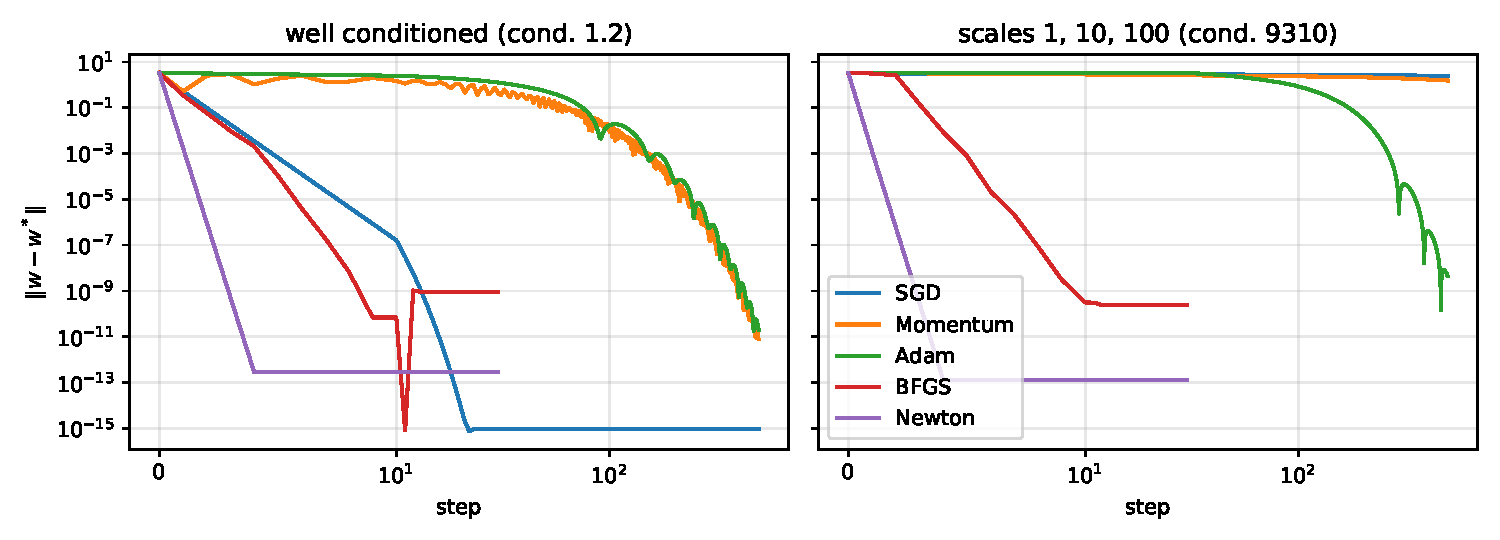
\includegraphics[width=\linewidth]{figures/linreg.pdf}
\caption{Distance to the closed-form solution at every step.}
\label{fig:linreg}
\end{figure}

With a condition number near 1 every method gets there, and plain gradient descent with
$\alpha = 1/L$ is among the fastest. With the features on different scales, the step that keeps the
steepest direction stable is far too small for the flattest one, and SGD and momentum are still
far from $w^*$ after 500 steps. Adam rescales every coordinate by its own gradient history, which
here largely undoes the scaling of the features. BFGS and Newton barely notice the conditioning:
damped Newton with a finite-difference Hessian is within $10^{-6}$ in a couple of steps on both
datasets, and BFGS needs a handful to learn the curvature.

% TODO(author): one or two sentences in your own words on what this says about first-order methods vs BFGS and Newton.

\subsection{MNIST}
\label{sec:mnist}

MNIST~\cite{lecun1998} has $60\,000$ training and $10\,000$ test images of $28\times28$ handwritten
digits. Pixels are scaled to $[0, 1]$. Two models, both trained with the engine:
\begin{itemize}
  \item \textbf{MLP}: $784 \to 256 \to 128 \to 10$, ReLU between layers.
  \item \textbf{CNN}: conv($1\to8$, $5\times5$, padding $2$), ReLU, max-pool $2\times2$,
        conv($8\to16$, $5\times5$, padding $2$), ReLU, max-pool $2\times2$, flatten, linear($784\to10$).
\end{itemize}
Both minimise the cross-entropy of Section~\ref{sec:losses} with Adam ($\alpha_0 = 10^{-3}$) on
minibatches of $64$, with the rate decaying linearly to $\alpha_0/100$ over the whole run
(\code{LinearDecay}). Every training minibatch is augmented: each digit is scaled by
$s \sim U(0.7, 1.3)$ about the centre and shifted by up to $13 - 10s$ pixels in each direction, so
that it stays inside the frame, by inverse mapping and bilinear interpolation~\cite{upc-ipa}; the
test set is not. The MLP is trained for 15 epochs and the CNN for 10. Each model is trained with
three seeds; test accuracy is measured once, at the end, on the float32 weights that are published
(the ones the website loads). The \emph{moved test} column is the same $10\,000$ test digits moved
and resized once in the same way, with a fixed seed.

\begin{table}[H]
\centering
\begin{tabular}{@{}lrrrlrr@{}}
\toprule
model & parameters & epochs & test accuracy (\%) & per seed & moved test (\%) & min / run \\
\midrule
MLP & 235,146 & 15 & $98.48 \pm 0.09$ & 98.49, 98.39, 98.56 & $97.38 \pm 0.02$ & 3.9 \\
CNN & 11,274 & 10 & $98.65 \pm 0.17$ & 98.85, 98.58, 98.53 & $97.49 \pm 0.20$ & 17.7 \\
\bottomrule
\end{tabular}
\caption{MNIST test accuracy, mean $\pm$ sample standard deviation over three seeds, on the test set as published and on the same digits moved and resized once with a fixed seed (moved test). Time is CPU training time in native Python.}
\label{tab:mnist}
\end{table}


The convolutional network is slightly more accurate with about $21\times$ fewer parameters: weight
sharing across positions builds in the translation structure that the MLP has to learn separately
for every pixel.

\begin{figure}[H]
\centering
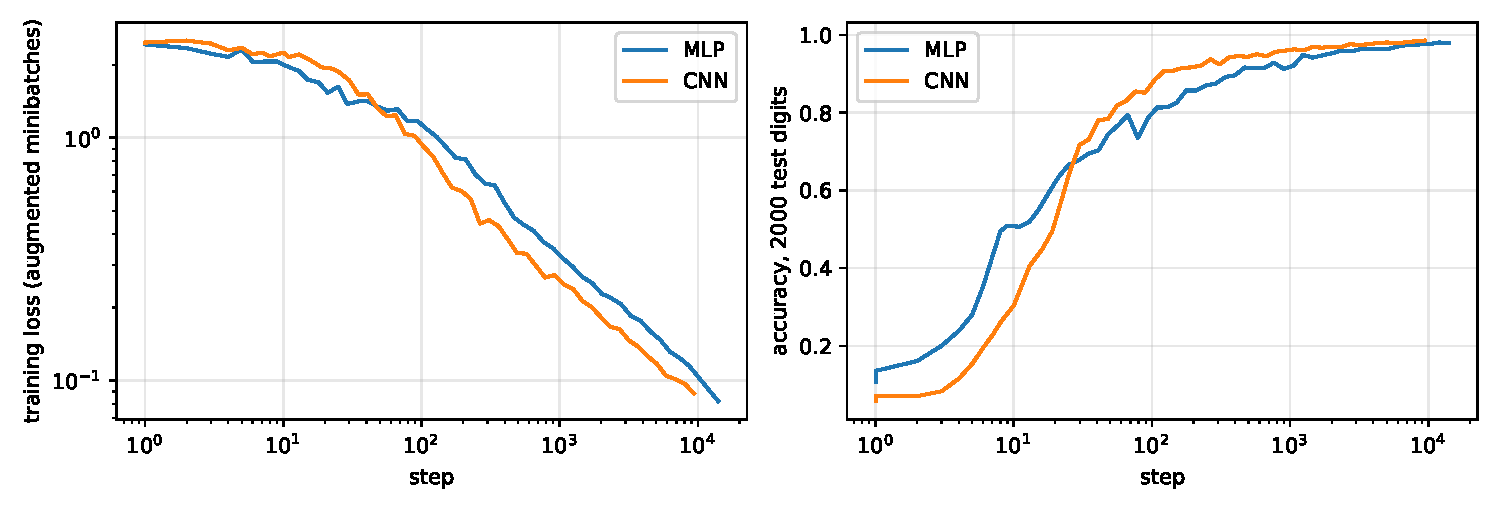
\includegraphics[width=\linewidth]{figures/mnist-curves.pdf}
\caption{Training loss (on the augmented minibatches) and accuracy on a fixed slice of $2\,000$ test
digits, at logarithmically spaced steps, for the published seed of each model.}
\label{fig:curves}
\end{figure}

Table~\ref{tab:shift} and Figure~\ref{fig:shift} give the test accuracy with every digit shifted
sideways, for the published models and for the same CNN trained without augmentation.

\begin{table}[H]
\centering
\begin{tabular}{@{}lrrrrrrrr@{}}
\toprule
 & \multicolumn{7}{c}{horizontal shift (pixels)} & \\
\cmidrule(lr){2-8}
model & $-6$ & $-4$ & $-2$ & $0$ & $+2$ & $+4$ & $+6$ & moved test \\
\midrule
CNN, no augmentation & 47.9 & 75.5 & 96.8 & 99.0 & 97.4 & 81.7 & 35.7 & 81.98 \\
CNN (published) & 93.2 & 97.5 & 98.4 & 98.9 & 98.5 & 97.2 & 88.9 & 97.72 \\
MLP (published) & 84.1 & 96.7 & 98.3 & 98.5 & 98.3 & 95.9 & 82.4 & 97.38 \\
\bottomrule
\end{tabular}
\caption{MNIST test accuracy (\%) with every digit moved sideways, and on the moved-and-resized test set of Table~\ref{tab:mnist}. The CNN without augmentation is the same network, seed and schedule as the published one, trained on the digits as they are; one seed.}
\label{tab:shift}
\end{table}


\begin{figure}[H]
\centering
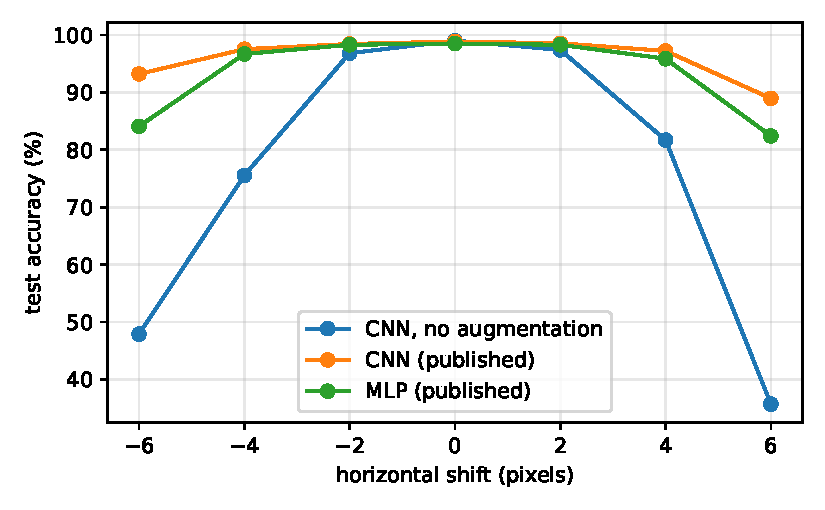
\includegraphics[width=0.6\linewidth]{figures/mnist-shift.pdf}
\caption{Test accuracy against a horizontal shift of every digit.}
\label{fig:shift}
\end{figure}
